\documentclass[table, 12pt]{article}
\usepackage[T1]{fontenc}
\usepackage[utf8]{inputenc}
\usepackage[english]{babel}
\usepackage{graphicx}
\usepackage{titlesec}
\usepackage{hyperref}
\usepackage[usenames,dvipsnames]{xcolor}
\usepackage{float}
\usepackage[export]{adjustbox}
\usepackage{longtable}
\usepackage{mathtools}
\usepackage[most]{tcolorbox}
\usepackage{xparse}
\usepackage{subcaption}

\hyphenation{Te-lan-ga-na}
\hyphenation{an-a-lys-ing}
\hyphenation{a-gron-o-mists}
\hyphenation{a-gron-o-mist}
\hyphenation{da-ta-base}
\hyphenation{ca-u-sed}
\hyphenation{Sen-sor-Da-ta-Ma-na-ger}
\hyphenation{Ac-count-Ma-na-ger}
\hyphenation{Lo-ca-tion-Mo-dule}
\titleformat{\paragraph}
{\normalfont\normalsize\bfseries}{\theparagraph}{1em}{}
\titlespacing*{\paragraph}
{0pt}{3.25ex plus 1ex minus .2ex}{1.5ex plus .2ex}


\def\exampletext{Example}

\NewDocumentEnvironment{testexample}{ O{} }
{
\colorlet{colexam}{teal!60!black} % Global example color
\newtcolorbox[use counter=testexample]{testexamplebox}{%
    % Example Frame Start
    empty,% Empty previously set parameters
    title={\exampletext #1},% use \thetcbcounter to access the testexample counter text
    % Attaching a box requires an overlay
    attach boxed title to top left,
       % Ensures proper line breaking in longer titles
       minipage boxed title,
    % (boxed title style requires an overlay)
    boxed title style={empty,size=minimal,toprule=0pt,top=4pt,left=3mm,overlay={}},
    coltitle=colexam,fonttitle=\bfseries,
    before=\par\medskip\noindent,parbox=false,boxsep=0pt,left=3mm,right=0mm,top=2pt,breakable,pad at break=0mm,
       before upper=\csname @totalleftmargin\endcsname0pt, % Use instead of parbox=true. This ensures parskip is inherited by box.
    % Handles box when it exists on one page only
    overlay unbroken={\draw[colexam,line width=.5pt] ([xshift=-0pt]title.north west) -- ([xshift=-0pt]frame.south west); },
    % Handles multipage box: first page
    overlay first={\draw[colexam,line width=.5pt] ([xshift=-0pt]title.north west) -- ([xshift=-0pt]frame.south west); },
    % Handles multipage box: middle page
    overlay middle={\draw[colexam,line width=.5pt] ([xshift=-0pt]frame.north west) -- ([xshift=-0pt]frame.south west); },
    % Handles multipage box: last page
    overlay last={\draw[colexam,line width=.5pt] ([xshift=-0pt]frame.north west) -- ([xshift=-0pt]frame.south west); },%
    }
\begin{testexamplebox}}
{\end{testexamplebox}\endlist}


\begin{document}
\begin{titlepage}
    \centering
    {\scshape\large AY 2021/2022 \par}
    \vfill
    
\includegraphics[width=100pt]{assets/logo-polimi-new.pdf}\par\vspace{1cm}
    {\scshape\LARGE Politecnico di Milano \par}
    \vspace{1.5cm}
    {\huge\bfseries Implementation Document \par}
    \vspace{2cm}
    {\Large {Ottavia Belotti\quad Alessio Braccini\quad Riccardo Izzo}\par}
    \vfill
    {\large Professor\par
        Elisabetta \textsc{Di Nitto}}
    \vfill
    {\large \textbf{Version 1.0}\\ \today \par}
\end{titlepage}

\hypersetup{%
    pdfborder = {0 0 0}
}

\thispagestyle{plain}
\pagenumbering{gobble}
\mbox{}
\newpage
\pagenumbering{roman}
\tableofcontents
\newpage
\pagenumbering{arabic}

\section{Introduction}
The code can be found in the official project repository on GitHub at the link: \url{https://github.com/AlessioBraccini/SE2-Belotti-Braccini-Izzo}.
\subsection{Purpose}

This document aims to describe how the implementation and integration
testing took place.
Implementation is the last step of the DREAM application
development cycle.
Testing, instead, means check that the critical parts of the application
works in a correct way, as described in the DD document.


\subsection{Definitions, Acronyms, Abbreviations}
\begin{itemize}
    \item ACID: Atomicity-Consistency-Isolation-Durability
    \item API: Application Programming Interface
    \item CSRF: Cross Site Request Forgery
    \item DBMS: DataBase Management System
    \item DD: Design Document
    \item HTTP: HyperText Transfer Protocol
    \item JS: JavaScript
    \item ORM: Object-Relational Mapping
    \item REST: REpresentational State Transfer
    \item RASD: Requirements Analysis and Specification Document
    \item UI: User Interface
    \item URL: Uniform Resource Locator
    \item WSGI: Web Server Gateway Interface
    \item ASGI: Asynchronous Server Gateway Interface
\end{itemize}
\subsection{Revision History}
\begin{itemize}
    \item Version 1.0:
\end{itemize}
\subsection{References}
\begin{itemize}
    \item Django Framework: \url{https://www.djangoproject.com/}
    \item REST Framework: \url{https://www.django-rest-framework.org/}
    \item Vue.js: \url{https://vuejs.org/}
    \item Axios: \url{https://axios-http.com/docs/intro}
\end{itemize}


\section{Development}
\subsection{Implemented Functionalities}
Given the three types of user, we decided to implement th functionalities for Policy Maker users and Agronomist user. In particular:
\subsubsection*{Policy Maker}
\begin{itemize}
    \item Farmers ranking
    \item Visualization of humidity sensors and water irrigation systems data as graphs
    \item Retrieving agronomists' reports about steering initiatives
\end{itemize}
\subsubsection*{Agronomist}
\begin{itemize}
    \item Farmers ranking tailored on the agronomist's district
    \item Uploading reports concerning steering initiatives
    \item Creation and updating of daily plans
    \item Help requests inbox
    \item Weather widget
\end{itemize}
\subsection{Adopted Development Frameworks}
Model-View-Controller paradigm

\begin{figure}
    \subfloat{{
\includegraphics[scale=0.05]{assets/Django-Logo.png}}}%
    \qquad
    \subfloat{{
\includegraphics[scale=0.4]{assets/Rest-Logo.png}}}%
    \caption{Django Framework and REST Framework logo}
\end{figure}
\subsubsection{Programming Language}
The programming language of choice for the DREAM backend is Python.

\begin{itemize}
    \item \textbf{Pros:}
    \begin{itemize}
        \item[+] \textbf{Allow fast development}: Python is a very high-level programming language, so the built-in functions and reliable third-parties libraries allow us to spend the development time focusing on implementing the desired custom behaviors rather than building basic and non-functional features that are shared among most web apps.
        \item[+] \textbf{Readability}: Python's syntax is very clear and human-friendly.
        \item[+] \textbf{Large community and widely spread among WebApps}: being used a lot by the web app developers' community, the internet is full of help for troubleshooting. Moreover, this has resulted in a very extensive support through libraries dedicated to web developing and integration with frontend frameworks.
    \end{itemize}
    \item \textbf{Cons:}
    \begin{itemize}
        \item[-] \textbf{Speed}: being an interpreted language, Python suffers of slower computation in comparison to other compiled languages (e.g. C++, Java, etc.).
    \end{itemize}
\end{itemize}

For the client side we chose JavaScript, a text-based programming language, that allows to build interactive web pages. It handles the user's interaction with the elements present on the page.
Alongside JavaScript, we used HTML and CSS to give structure and style to the page.

\subsubsection{Django Framework}
Django is Python web framework whose key is rapid development without sacrificing well structured code. In fact, the framework encourages to follow the MVC pattern and embeds it into its Django apps structure.

It is \textbf{secure}, since it provides the developers security tools (e.g. automatic user's passwords encryption, CSRF protection, SSL/HTTPS support, etc.) that have been implemented by experts in the field. See more about security in section \ref{REST}.

It is \textbf{supportive}, given that it has lots of database operation support thanks to the \emph{Object-relational mapping} (ORM) feature which easily maps DB tables to \emph{Django Model} components (Model in MVC pattern) within the code, basic queries can be done transparently and in a very readable fashion without losing in performance. Moreover, it allows to configure the \emph{Admin Interface} from where we, as backend developers, can easily manage the database, like monitoring at a glance the entries in all the DB tables and create new ones for testing purposes. A part from the DB integration,  Django allows the creation of custom \emph{endpoint URLs} from where the frontend will make the backend calls. Meanwhile the \emph{Django View} components come to be a dedicated place for managing HTTP requests, acting as the Controller in MVC design. Django would also support \emph{Template} components as its Views in MVC pattern, but in this project it hasn't been used because of the different framework choice to handle the presentaion part (see section \ref{Vue}). 

Furthermore, Django is \textbf{extensively documented} and \textbf{scalable} since it's being used in very demanding professional contexts, being one of the frameworks of choice of well known social media platforms that experience high loads of requests due to their intensive usage from their user base.

\subsubsection{Django REST Framework}
\label{REST}
We decided to pair REST framework to our Django backend since REST allows even more security features.

We used its authentication policies, in particular the \textbf{REST Token-based authentication} that ensures an authorized clients' connection to the backend, so that every interaction with the application server is safe from an authentication point of view: unknown users can access none of the backend's functionalities.

We used the \emph{Djoser} REST library to handle users login and signup. The choice has been taken to make sure that such standard operations are carried out without flaws, especially in handling sensitive data (i.e. passwords). Moreover, \emph{Djoser} is compatible with custom User Models, so it enables us to delegate the authentication phase to it even with our custom User model.

Furthermore, Django REST gives an extensive support in building \emph{Django Views}, from basic skeleton function (\texttt{@api\_view}) for managing all types of HTTP requests, up to more functional and request-specific functionalities.

\subsubsection{Vue.js}
\label{Vue}
Vue.js is an open-source model–view–viewmodel front end JavaScript framework that allow to create user interfaces and single-page applications.
Vue.js features an incrementally adaptable architecture that focuses on declarative rendering and component composition.
The core library is focused on the view layer only.
Advanced features required for complex applications such as routing, state management and build tooling are offered via officially maintained supporting libraries and packages.

We used this framework to build up the client-side rendering of pages because its easy usage as it integrate in a single .vue file, also called components,
the HTML, CSS and javascript part.

In order to communicate with the backend we use the javascript library Axios.
It is a promise-based HTTP Client for node.js and the browser.
On the server-side it uses the native node.js http module, while on the client it uses XMLHttpRequests.
It transforms in an automatic way the json reply that arrives from the server in vue ready XMLHttpRequests.

\subsection{API Integration}
\subsubsection{OpenWeatherMap API}
To allow the user to retrieve the weather information we use this external api service that let us know in real time
the weather condition of a specific territory.
This return us not only the basics information but also more specific ones.

\subsection{DataBase}
Our database system of choice is PostgreSQL, a well known object-relational database. It is reliable, robust, ACID-compliant and ensures high performance. 

\section{Source Code}
\subsection{Backend Structure}
\begin{center}
    \begin{figure}[H]
        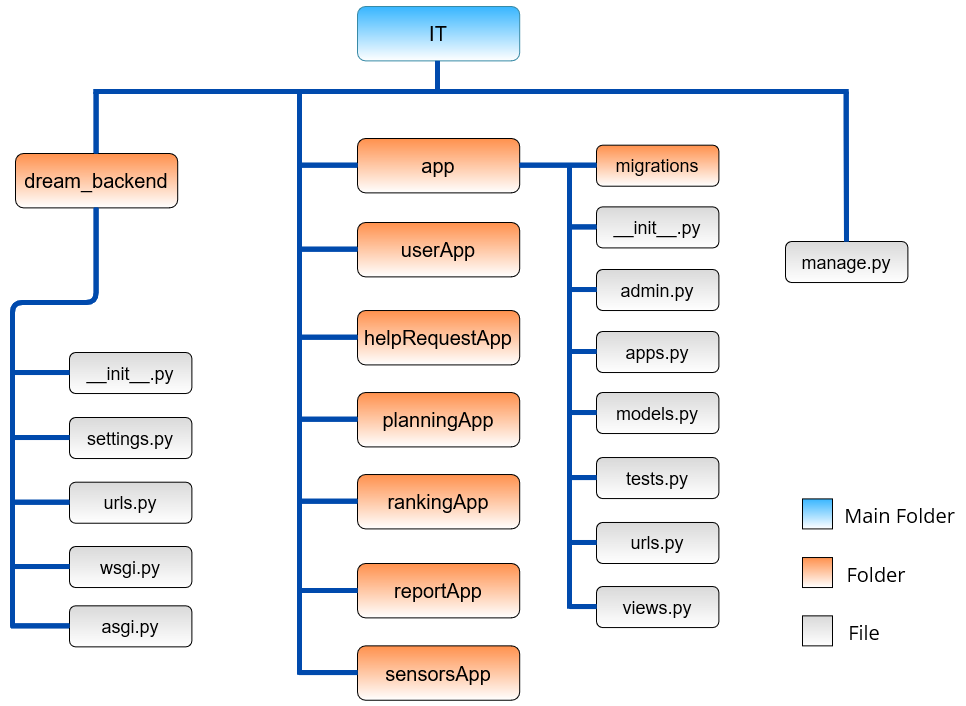
\includegraphics[scale=0.65, center]{assets/backend_structure.png}
        \caption{Backend structure}
        \label{fig: backend_structure}
    \end{figure}
\end{center}

% basic description
The back-end of the application follows the common Django project structure as shown in the figure above.
This section describes the structure of the project and the role of each app.\newline
Here is represented the structure of the back-end:

\begin{itemize}
    \item \textbf{IT}: root directory, container for the project
    \item \textbf{dream\_backend}: folder that contains the configuration files of the project
    \item \textbf{\_\_init.py\_\_}: it tells the Python interpreter that the directory is a Python package
    \item \textbf{settings.py}: main setting file for the Django project, used to configure all the applications and middleware, it also handles the database settings
    \item \textbf{urls.py}: URL declarations for the Django project, it contains all the endpoints that the website should have
    \item \textbf{wsgi.py}: entry-point for WSGI-compatible web servers to serve your project, it describes the way how servers interact with the applications
    \item \textbf{asgi.py}: entry-point for ASGI-compatible web servers to serve your project, ASGI works similar to WSGI but comes with some additional functionality
    \item \textbf{migrations}: Django's way of propagating changes to the models into the database schema, when changes occur this folder is populated with the records of them
    \item \textbf{admin.py}: used for registering the Django models into the Django administration, it allows to display them in the Django admin panel
    \item \textbf{apps.py}: common configuration file for all Django apps, used to configure the attributes of the app
    \item \textbf{models.py}: it defines the structure of the database, it allows the user to create database tables for the app with proper relationships using Python classes. It tells about the actual design, relationships between the data sets and their attribute constraints
    \item \textbf{tests.py}: used to test the overall working of the app through unit tests
    \item \textbf{views.py}: provide an interface through which a user interacts with a Django website, it contains the business logic of the app
    \item \textbf{manage.py}: command-line utility for executing Django commands; these includes debugging, deploying and running
\end{itemize}

\begin{center}
    \begin{figure}[H]
        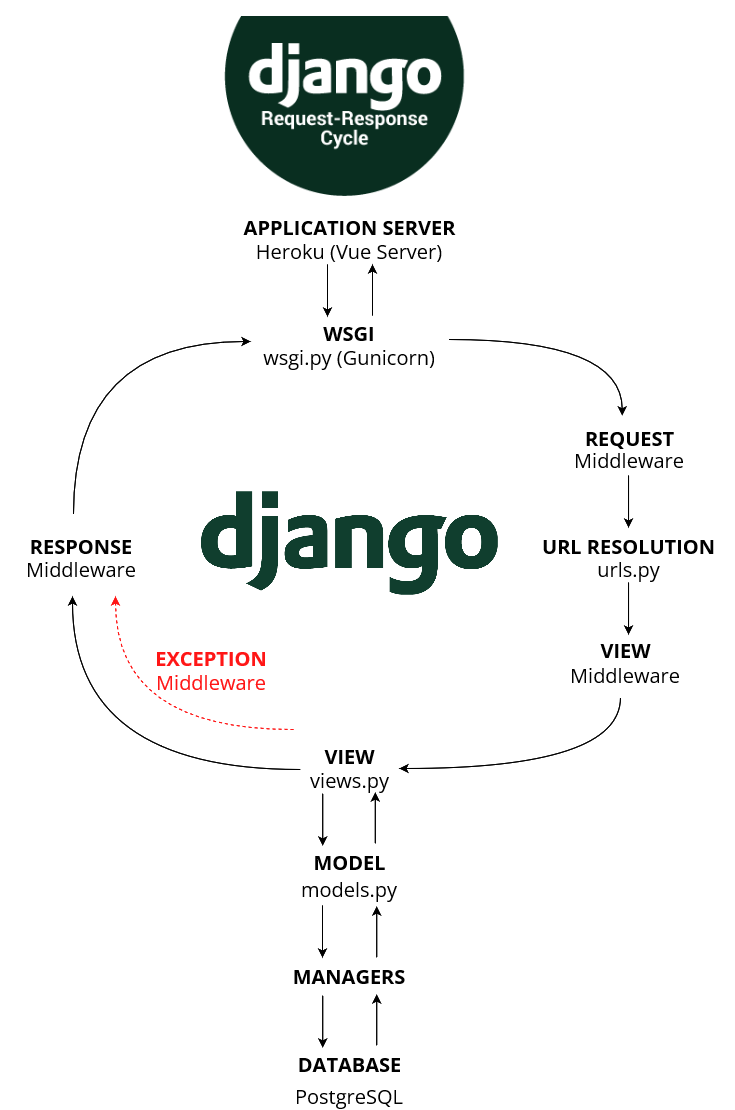
\includegraphics[scale=0.55, center]{assets/django_request_response_flow.png}
        \caption{Django Request-Response Cycle}
        \label{fig: django_flow}
    \end{figure}
\end{center}

% describe apps
All the functionalities of the website are managed by different apps, these are the ones implemented:
\begin{itemize}
    \item \textbf{app}: implements common functionalities that cover the entire application, it has one endpoint:
    \begin{itemize}
        \item[--] \textbf{farms\_list}: handled by \textit{FarmView} view, it manages GET requests by returning a list of farms
    \end{itemize}
    \item \textbf{userApp}: implements the custom authentication system of the application, it contains all the models regarding the user. It has one endpoint that is used to check if a user is authenticated or not
    \item \textbf{helpRequestApp}: implements the functionalities about the help requests with two endpoints:
    \begin{itemize}
        \item[--] \textbf{help\_request}: handled by \textit{HelpRequests} view, it manages GET requests by returning the list of help requests and POST requests to reply to an existing requests
        \item[--] \textbf{help\_request\_by\_id}: handled by \textit{HelpRequestByID} view, it manages GET requests by returning a single help request associated to the unique id specified as a parameter
    \end{itemize}
    \item \textbf{planningApp}: implements the functionalities about the daily plan with two endpoints:
    \begin{itemize}
        \item[--] \textbf{daily\_plan}: handled by \textit{DailyPlanView} view, it manages GET requests by returning the list of dates for the daily plan and POST requests to upload a new daily plan
        \item[--] \textbf{update\_daily\_plan}: handled by \textit{UpdateVisits} view, it manages GET requests by returning the list of farmers in the current daily plan and POST requests to perform an update of an already existing daily plan
    \end{itemize}
    \item \textbf{rankingApp}: implements the functionalities about the ranking with two endpoints:
    \begin{itemize}
        \item[--] \textbf{rank\_farmers}: handled by \textit{RankFarmers} view, it manages GET requests by returning the ranking as a list of farmers
        \item[--] \textbf{profile\_info}: handled by \textit{ProfileFarmers} view, it manages GET requests by returning the profile info of a selected farmer
    \end{itemize}
    \item \textbf{reportApp}: implements the functionalities about the steering initiatives with two endpoints:
    \begin{itemize}
        \item[--] \textbf{steering\_initiatives}: handled by \textit{SteeringInitiativeView} view, it manages GET requests by returning the list of reports uploaded to the app and POST requests to upload a new report
        \item[--] \textbf{download\_reports}: handled by \textit{DownloadReport} view, it manages GET requests by returning a specific reports based on some parameters
    \end{itemize}
    \item \textbf{sensorsApp}: implements the functionalities about the sensors (humidity and water irrigation) with two endpoints:
    \begin{itemize}
        \item[--] \textbf{humidity}: handled by \textit{Humidity} view, it manages GET requests by returning a list with humidity and temperature values for each district
        \item[--] \textbf{water\_irrigation}: handled by \textit{WaterIrrigation} view, it manages GET requests by returning a list of water quantity values for each district
    \end{itemize}
\end{itemize}
% flow of requests

\subsection{Frontend Structure}

The front-end web application is contained into the dream\_frontend folder of
the IT directory.
Of course, following the four tier architecture described in the Design Document,
the front-end web application can also be deployed to a dedicated web server,
which will then make requests to a different backend server.
Here is represented the structure of the web app:



\newpage
\section{Testing}

In this section we described how we tested the application following the general guidelines given in the Design Document.
The testing process has been divided into unit testing and integration testing.
We decided to test only the back-end because most of the logic resides here.
In any case, the system testing and the post-deployment testing phases also covered the functioning of the front-end.

\subsection{Unit Testing}
For each app in the back-end we wrote the test cases in tests.py file using \textbf{unittest}, a built-in module from the Python standard library.
\subsubsection*{helpRequestApp}
\begin{itemize}
    \item Attempt to get the list of help requests by a user through a GET request on \textit{help\_request} endpoint
    \item Attempt to get the list of help requests in case of an invalid user
    \item Attempt to reply to an existing help request through a POST request on \textit{help\_request} endpoint, verify the correct deletion of the old help request which is replaced by the reply
    \item Attempt to reply to an existing help request in case of an invalid user
    \item Attempt to get a single help request given the id through a POST request on \textit{help\_request\_by\_id} endpoint
    \item Attempt to get a single help request given the id in case of an invalid user
\end{itemize}
\subsubsection*{planningApp}
\begin{itemize}
    \item Attempt to upload a new daily plan through a POST request on \textit{daily\_plan} endpoint
    \item Attempt to upload a new daily plan with an invalid region
    \item Attempt to upload a new daily plan with an invalid date
    \item Attempt to upload a new daily plan with an duplicated farmer
    \item Attempt to upload a new daily plan with an invalid user (not an agronomist)
    \item Attempt to retrieve the daily plans through a GET request on \textit{daily\_plan} endpoint
    \item Attempt to retrieve only the daily plans associated to the current user
    \item Attempt to update a daily plan through a POST request on \textit{update\_daily\_plan} endpoint
    \item Attempt to update an old daily plan
    \item Attempt to remove a daily plan
    \item Attempt to update a daily plan before creating it
\end{itemize}
\subsubsection*{rankingApp}
\begin{itemize}
    \item Attempt from an agronomist to get the ranking with "descending" order specified in the parameters through a GET request on \textit{rank\_farmers} endpoint
    \item Attempt from an agronomist to get the ranking with "ascending" order specified in the parameters
    \item Attempt from a policymaker to get the ranking with "descending" order and district among the parameters
    \item Attempt from a policymaker to get the ranking with "ascending" order and district among the parameters
    \item Attempt from a policymaker to get the ranking with different districts
    \item Attempt from a policymaker to get the ranking with "ascending" order but without the district among the parameters
    \item Attempt from a policymaker to get the ranking with "descending" order but without the district among the parameters
    \item Attempt to get informations about a farmer in the ranking through a GET request on \textit{profile\_info} endpoint
    \item Attempt to get informations about a farmer in the ranking in case of an invalid user
\end{itemize}
\subsubsection*{reportApp}
\begin{itemize}
    \item Attempt from an agronomist to upload a new report through a POST request on \textit{steering\_initiatives} endpoint
    \item Attempt from a policymaker to upload a new report
    \item Attempt to upload duplicated reports
    \item Attempt to get the list of reports through a GET request on \textit{steering\_initiatives} endpoint
\end{itemize}
\subsubsection*{sensorsApp}
\begin{itemize}
    \item Attempt to get data about humidity sensors through a GET request on \textit{humidity} endpoint
    \item Attempt to get data about water irrigation sensors through a GET request on \textit{water\_irrigation} endpoint
\end{itemize}

There is a total of 32 tests with a percentage of success of 100\%, this establishes the stability of the system.
All the tests can be verified by running "python manage.py test" in the root directory.

\subsection{System Testing}
A part of the testing phase was also dedicated by manually testing the app through the web browser and with Postman, a tool for making HTTP GET/POST requests with custom parameters.
In this way we tested the authentication phase and all the functionalities provided by the system.
All the tests have been performed successfully.

\subsection{Post-deployment Testing}
After the deploy the application has been extensively tested on a daily basis. This allowed to test the entire system and the interactions between the components both on front-end and back-end.
We also invited a couple of testers in order to stress the app.


% \section{Build} %don't really have to build


\section{Installation}
\subsection{Requirements}
\subsection{Backend Installation}
\subsection{Frontend Installation}

\section{Effort Spent}
\begin{tabular}{|c||c|}
    \hline
    Student & Time for implementation\\ \hline
    Ottavia Belotti & 80h\\
    Alessio Braccini & 80h\\
    Riccardo Izzo & 80h\\
    \hline
\end{tabular}

\end{document}

